\documentclass[11pt]{scrartcl}

\RequirePackage{selinput}
\RequirePackage{layouts}
\RequirePackage{printlen}
\RequirePackage{calculator}
\RequirePackage{geometry}
\RequirePackage{enumitem,varwidth}
\RequirePackage[svgnames]{xcolor}
\RequirePackage{tikz}
\RequirePackage{pgf-pie}
\RequirePackage{lmodern}
\RequirePackage{environ}
\RequirePackage{wrapfig}
\RequirePackage{fdsymbol}
\RequirePackage{fontawesome}
\RequirePackage{graphicx}
\RequirePackage{siunitx}
\RequirePackage{csquotes}
\RequirePackage[gen]{eurosym}
\RequirePackage{caption}
\usetikzlibrary{shapes.geometric}

\captionsetup[figure]{name={}}

\usepackage{mathtools}
\SetLabelAlign{center}{\clap{#1}}

\geometry{
 a4paper,
 left=15mm,
 top=10mm,
 right=10mm,
 bottom=10mm
}
\pagestyle{empty}
\setlist{itemsep=-0.2em} % or \setlist{noitemsep} to leave space around whole list
\graphicspath{ {./img/} }


\newcommand{\swotWidth}{18}
\newcommand{\swotHeight}{8}
\DIVIDE{\swotWidth}{2}{\tileWidth}
\DIVIDE{\swotHeight}{2}{\tileHeight}
\DIVIDE{\tileWidth}{2}{\xTile}
\DIVIDE{\tileHeight}{2}{\yTile}

\parindent0em

\begin{document}

\sisetup{
    group-separator = {,},
    group-minimum-digits = 4
}



% %%%%%%%%%%%%%%%%%%%%%%%%%%
% Company sheet Title
% %%%%%%%%%%%%%%%%%%%%%%%%%%
\begin{minipage}{\textwidth}
    % %%%%%%%%%%%%%%%%%%%%%%%%%%
    % Title
    % %%%%%%%%%%%%%%%%%%%%%%%%%%
    \center
\includegraphics[width=2em]{company_logo.png}
    {\textbf{Mensch und Maschine}}
\end{minipage}\\



% %%%%%%%%%%%%%%%%%%%%%%%%%%
% Company Story and Information
% %%%%%%%%%%%%%%%%%%%%%%%%%%

\begin{minipage}[t]{0,73\linewidth}
    The german company \enquote{Mensch und Maschine} resells CAD/E/M
    products by the american company \enquote{AutoDesk} and develops
    own features and Add-ons. The attractive growth in sales, margins
    and dividend needs o continues to be a very good investment. The
    two-pillar business model of a high margin software development and
    lower-margin VAR/project business adds up pretty nicely. Over the
    coming years, M+M must increase it's margins and find ways to reduce
    costs, especially in the VAR-Segment! But the strong balance sheet,
    over 30 years of experience and low exposure to institutional investors
    makes it a great Peter Lynch story.
\end{minipage}\hfill
\begin{minipage}[t]{0,23\linewidth}
    \begin{itemize}[wide, labelsep = 1em, align=center]\scriptsize
        \item [\faAsterisk] 1984
        \item [\faMale] Adi Drotleff
        \item [\faEuro] \faEuro \num{24.594} m
        \item [\faUsers] \num{946}
        \item [\faIndustry] CAD-Software
        \item [\faBook] \faEuro \num{73,515} m
        \item [\reflectbox{\rotatebox[origin=c]{270}{\faLevelDown}}] \faEuro
        \item [\faFolderOpen]Fast grower
        \item [\faQuestion]
        \begin{enumerate}
            \item Fast grower
            \item Long time dividend payer
            \item Growing Dividend 20\%
        \end{enumerate}
    \end{itemize}
\end{minipage}


% %%%%%%%%%%%%%%%%%%%%%%%%%%
% Additional information
% %%%%%%%%%%%%%%%%%%%%%%%%%%
    \begin{minipage}{.6\linewidth}
        \faArchive\space\textbf{Products:}
        \begin{enumerate}
            \item Claims to reduce production times
            \item over 100 proucts in CAD/M/E
        \end{enumerate}
        $\Rightarrow$ Needed for building Bridges, Gardens, stadiums, manufacturing
    \end{minipage}
    \begin{minipage}{.4\linewidth}
        \centering
            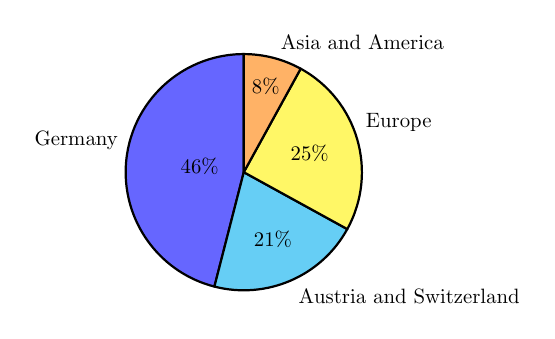
\begin{tikzpicture}[scale=.75, every node/.style={scale=.75}] % Tikz environment
                \pie[rotate=90, radius=2]
                {46/Germany, 21/Austria and Switzerland, 25/Europe, 8/Asia and America}
            \end{tikzpicture}
        \captionof*{figure}{Revenue 2019}
    \end{minipage}
    \begin{minipage}{.4\linewidth}
        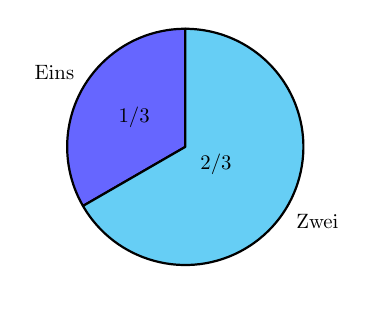
\begin{tikzpicture}[scale=.75, every node/.style={scale=.75}]
            \pie[sum=auto, rotate=90, radius=2]
            {{1/3}/Eins, {2/3}/Zwei}
        \end{tikzpicture}
    \end{minipage}





% %%%%%%%%%%%%%%%%%%%%%%%%%%
% SWOT
% %%%%%%%%%%%%%%%%%%%%%%%%%%
\begin{tikzpicture}[
    square/.style={%
        shape=rectangle, minimum width=\tileWidth cm, minimum height=\tileHeight cm,
        inner sep=-1mm, draw
    }, font=\scriptsize\sffamily, thick
]
% \draw[help lines] (-16,-16) grid (16,16);
\draw[black, fill=gray] (-\tileWidth,-\tileHeight) rectangle (\tileWidth,\tileHeight);



% Strengths %
\node [square, fill=DarkSeaGreen!75!yellow, text width=\tileWidth cm] at (-\xTile,\yTile) {
    \begin{varwidth}{\linewidth}
        \begin{itemize}[leftmargin=*,noitemsep]
            \item Lead by founder Adi Drotleff
            \item Grew profitable with new issuance of shares - Buyback of \num{80592} shares @\euro\num{33,22}
            \item No customer accouts for more than 2\% of revenue
            \item Management owns  over 50\% of the company
            \item Strong balance sheet, ~\euro\num{15}m in debt, \euro\num{32}m CashFlow (9M 2020)
        \end{itemize}
    \end{varwidth}
};

% Weaknesses
\node [square, fill=red!25, text width=\tileWidth cm] at (\xTile, \yTile) {
    \begin{varwidth}{\linewidth}
        \begin{itemize}[leftmargin=*,noitemsep]
            \item Increased outstanding shares: 2014: \num{15439}m to 2019: \num{16820}m shares
            \item Heavily relying on AutoDesk price policy
            \item VAR business expansion into other countries requires new offices $\rightarrow$ costs
            \item Strong Focus in \enquote{D/A/CH} region, maybe too much
            \item Personel risks, specific knowledge is required
        \end{itemize}
    \end{varwidth}
};

% Opportunities
\node [square, fill=DarkSeaGreen!75, text width=\tileWidth cm] at (-\xTile,-\yTile) {
    \begin{varwidth}{\linewidth}
        \begin{itemize}[leftmargin=*,noitemsep]
            \item Germany requires BIM-enabled 3D models for public building projects
            \item High-margin internally developed software
            \item Economics of scale in VAR buisiness $\rightarrow$ Higher margins lead to lower costs
        \end{itemize}
    \end{varwidth}
};

\node [square, fill=Salmon!75, text width=\tileWidth cm] at (\xTile,-\yTile) {
    \begin{varwidth}{\linewidth}
        \begin{itemize}[leftmargin=*,noitemsep]
            \item Autodesk main supplier in VAR Segment
            \item Heavily reliant on VAR business (roughly \num{70}\%)
            \item High cost, overhead for VAR business $\rightarrow$ low margins
            \item Takes further capital increases into consideration (For what?!)
        \end{itemize}
    \end{varwidth}
};

\draw(-0.3,0.3) node {\large\textbf{S}};
\draw(0.3,0.3) node {\large\textbf{W}};
\draw(-0.3,-0.3) node {\large\textbf{O}};
\draw(0.3,-0.3) node {\large\textbf{T}};

\end{tikzpicture}

\end{document}